% CS 455, FA'24 Software Design Document template
% Software design template based on the template from
% Shared Password Manager
% https://tex.stackexchange.com/questions/42602/software-requirements-specification-with-latex
\documentclass[letterpaper,12pt,oneside,listof=totoc]{scrreprt}
\usepackage{listings}
\usepackage{underscore}
\usepackage{xcolor}
\definecolor{purple}{rgb}{0.5, 0, 0.5} % Adjust the RGB values as needed
\usepackage{graphicx}
\usepackage{tabularx} % Add this to your preamble
\usepackage{array} 
\usepackage[margin=1.25in]{geometry}
\usepackage[bookmarks=true]{hyperref}

\usepackage{booktabs}
\usepackage{tikz}
\def\checkmark{\tikz\fill[scale=0.4](0,.35) -- (.25,0) -- (1,.7) -- (.25,.15) -- cycle;}

\hypersetup{
    bookmarks=false,                                % show bookmarks bar
    pdftitle={Software Design Document}, % title
%    pdfauthor={Yiannis Lazarides},                  % author
%    pdfsubject={TeX and LaTeX},                     % subject of the document
%    pdfkeywords={TeX, LaTeX, graphics, images},     % list of keywords
    colorlinks=true,                                % false: boxed links; true: colored links
    linkcolor=blue,                                 % color of internal links
    citecolor=black,                                % color of links to bibliography
    filecolor=black,                                % color of file links
    urlcolor=purple,                                % color of external links
    linktoc=page                                    % only page is linked
}%
\def\myversion{1.0 }
\date{\today}
\author{} % suppress warning, do not fill this in
\begin{document}
% we don't use \maketitle because we overide the default title page here
\begin{titlepage}
\flushright
\rule{\textwidth}{5pt}\vskip1cm
\Huge{SOFTWARE DESIGN DOCUMENT}\\
\vspace{1.5cm}
for\\
\vspace{1.5cm}
Shared Password Manager System\\                      %%% Update the title page text
\vspace{1.5cm}
\LARGE{Release 1.0\\}
\vspace{1.5cm}
\LARGE{Version \myversion approved\\}
\vspace{1.5cm}
Prepared by The Better Team\\
\vfill
\rule{\textwidth}{5pt}
\end{titlepage}
\tableofcontents
\listoffigures
\listoftables

\chapter*{Revision History}
% Update this table for each approved revision of the design starting with the baseline
% Add the new content followed by a \hline

\begin{tabular}{| c | p{0.60\textwidth} | p{0.30\textwidth} |}
\hline
Date     & Description   & Revised by \\
\hline
11-08-2024 & First Baseline & James A. Jerkins \\
11-19-2024 & Second Baseline & James A. Jerkins \\
12-8-2024 & Third Baseline & James A. Jerkins \\
\hline
\end{tabular}

% What is a Software Design Document (SDD)?
%
% Software design is a process by which the software requirements are translated into a representation of software components, interfaces, and data necessary for the implementation phase. The SDD shows how the software system will be structured to satisfy the requirements. It is the primary reference for code development and, therefore, it must contain all the information required by a programmer to write code. The SDD is typically performed in two stages. The first is a preliminary design in which the overall system architecture and data architecture is defined. In the second stage -- i.e., the detailed design stage -- more detailed data structures are defined and algorithms are developed for the defined architecture.
%
% This template is an annotated outline for a software design document adapted from the IEEE Recommended Practice for Software Design Descriptions. The IEEE Recommended Practice for Software Design Descriptions have been reduced in order to simplify this assignment while still retaining the main components and providing a general idea.
%

\chapter{INTRODUCTION}

\section{Purpose}
%Identify the purpose of this SDD and its intended audience. (e.g. ``This software design document describes the architecture and system design of XX ...'').
The Software Design Document (SDD) for the Shared Password Manager application offers a comprehensive overview of the architecture and system design to securely manage user stored credentials. 

\section{Scope}
The Shared Password manager system design will make use of a website application environment to provide functionality for three types of users to interact with the system: admin, regular, and view-only. 
To use the application, a user will first login to their account. The Application will then display options dependent on their privilege level. For admin users, they will have the ability to add/remove users, while regular users will have the functionality to view, add, and edit entered credentials. Additionally, View-only users will only have privilege to view credentials. The User Data will be stored securely in an SQLite database using a server. 

\section{Overview}
%Provide an overview of this document and its organization. This section describes how to read and use this document.
This documents contains sections that describes the necessary components and sections that describe sub systems for the Shared password Manager system. This document should be used to understand the underlying components to communicate the intention of each systems with stakeholders. This document also serves as a troubleshooting guide to developers tasked with modifying and maintaining availability of the software.

\section{References}
[1] WT documentation, “A hands-on introduction to Wt::Dbo by Matthias, "
\newline https://www.webtoolkit.eu, 2024. (accessed Oct. 21, 2024) \newline
\url{https://www.webtoolkit.eu/wt/doc/tutorial/dbo.html}\newline

\section{Definitions and Acronyms}
%This section is optional. Provide definitions of all terms, acronyms, and abbreviations that the reader may need to know to properly understand this SDD. These definitions should be items used in the SDD that are most likely not known to the audience. Common acronyms do not need to be included.

\section{Acronyms}
\addcontentsline{lot}{table}{Acronym table} % Add table to list of tables manually
\begin{tabular}{| c | p{0.80\textwidth}|}
\hline
Acronym & Meaning\\
\hline
enum & enumerated type \\
\hline
MVC & Model-View-Controller Architecture \\
\hline
\end{tabular}
 \newline
 
\chapter{SYSTEM OVERVIEW}
%Give a general description of the functionality, context, and design of your project. Provide any background information if necessary.
The Shared Password manager system is an application with the purpose of storing user's password credentials. A user can log into their account and access the logged credentials so the user is not burdened with remembering password credentials. The system requires an admin user to control and manage user groups. 

\chapter{SYSTEM ARCHITECTURE}
\section{Architectural Design}
%Develop a modular program structure and explain the relationships between the modules to achieve the complete functionality of the system. This is a high level overview of how responsibilities of the system are partitioned and then assigned to subsystems. Identify each high level subsystem and the roles or responsibilities assigned to it. Describe how these subsystems collaborate with each other in order to achieve the desired functionality. Don't go into too much detail about the individual subsystems. The main purpose is to gain a general understanding of how and why the system was decomposed, and how the individual parts work together. Provide a diagram showing the major subsystems and data repositories and their interconnections. Refer to and describe the diagram in the narrative.
The Shared Password manager system will use a Model-View Controller (MVC) Architecture style as presented in figure~\ref{arch}. This Model is responsible for handling the logic upon the data and interacts with the database. The View is responsible displaying. Lastly, the Controller is responsible for only handling request flows from the view and model logical units. 


\begin{figure}
\centering
\makebox[\textwidth][c]{%
  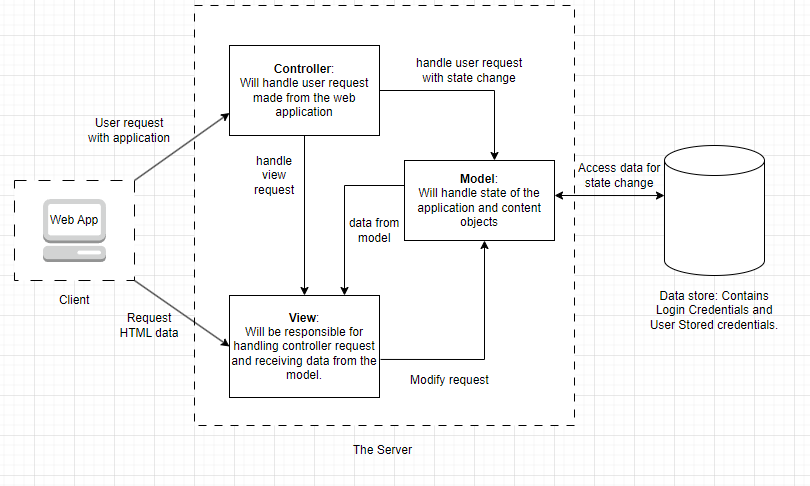
\includegraphics[width=1.4\textwidth]{arch.png}
}
\caption{MVC Architecture diagram}
\label{arch}
\end{figure}


\section{Decomposition Description}
%Provide a decomposition of each one of the subsystems in the architectural design. You may choose to give a functional description or an object oriented (OO) description. For a functional description use appropriate diagrams such as top-level data flow diagrams (DFD) and structured decomposition diagrams. For an OO description use the appropriate diagrams such as subsysterm model, object digrams, generalization diagram(s), aggregation diagram(s), interface, and specification diagrams.
The Model-View Architecture chosen has been broken down into several components as presented in figure~\ref{class1}. The View Component of the system is responsible for connecting the User interface to a client request to the model. The Model component of the diagram is responsible for handling the user's request and making the necessary database request to the SQLite database. 

%The User class component represents the model functionality of the system. The Web\_interface component contains functionality for the presentation of the User Interface. Lastly, the controller is represented with the Request encryptor class which is responsible for handling the user's request between the model and view components.

\begin{figure}
\centering
\makebox[\textwidth][c]{%
  \includegraphics[width=1.5\textwidth]{class1.png}}
\caption{Class diagram}
\label{class1}
\end{figure}

\begin{figure}
\centering
\makebox[\textwidth][c]{%
  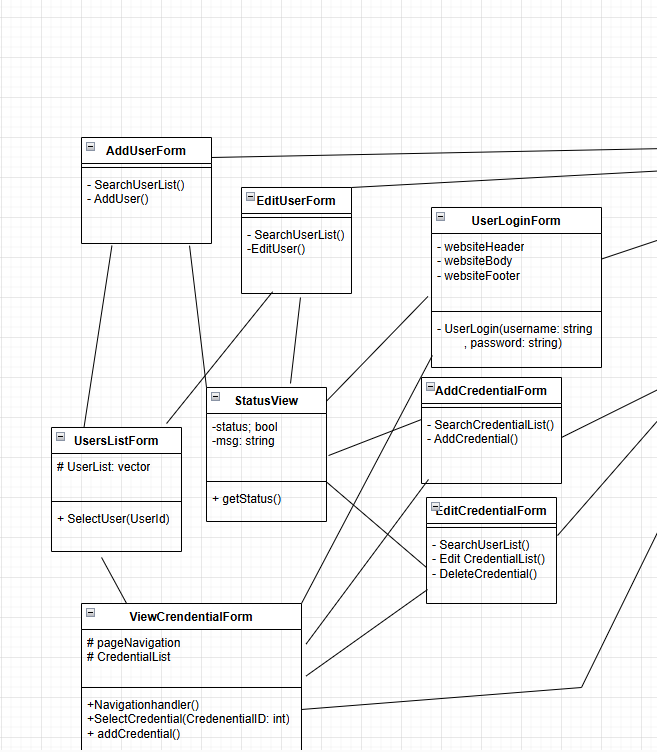
\includegraphics[width=1.0\textwidth]{class2.png}}
\caption{View - Class diagram}
\label{class3}
\end{figure}

\begin{figure}
\centering
\makebox[\textwidth][c]{%
  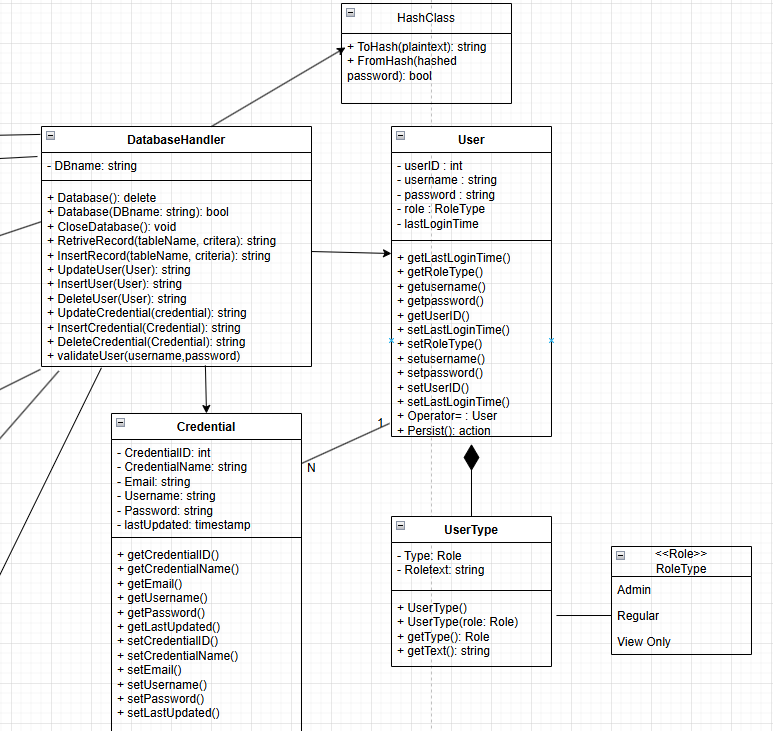
\includegraphics[width=1.0\textwidth]{class3.png}}
\caption{Model - Class diagram}
\label{class2}
\end{figure}


\section{Design Rationale}
%Discuss the rationale for selecting the architecture described in the previous section including critical issues and trade/offs that were considered. You may discuss other architectures that were considered, provided that you explain why you didn't choose them.
% NOTE: Since webtoolkit is a customer constraint (required), the architecture is strongly influenced by Witty.
The Model View Architecture is a commonly used to create web based applications. No other architecture styles were considered due to chosen style has already proven viable for web applications. A design trade off with the chosen architecture, is the model module will handle the user request to the view and model.  


\chapter{DATA DESIGN}
\section{Data Description}
%Explain how the information domain of your system is transformed into data structures. Describe how the major data or system entities are stored, processed and organized.
The data design for the Shared password manager is centered about User Data and User Credential data storage. 
The Entity-Relation(E/R) diagram \ref{arch} depicts how the data is stored and logically separated between user types.


\begin{figure}
\centering
\makebox[\textwidth][c]{%
  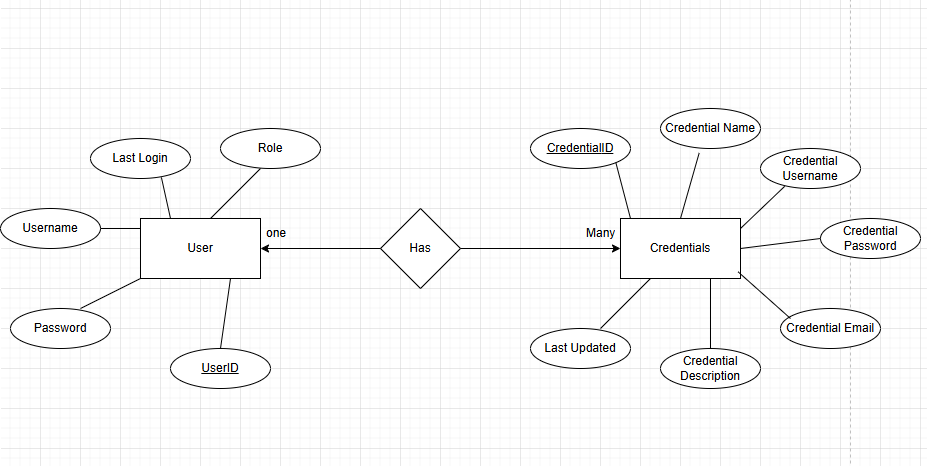
\includegraphics[width=1.2\textwidth]{ER.png}
}
\caption{E/R diagram}
\label{arch}
\end{figure}


\section{Data Dictionary}
%Alphabetically list the system entities or major data along with their types and descriptions. If you provided a functional description in the ``Decomposition'' Section, list all the functions and function parameters. If you provided an OO description, list the objects and the associated attributes, methods and method parameters.
Credential:\newline
-ID\newline
-name\newline
-email\newline
-username\newline
-password\newline
-description\newline
User:\newline
-ID\newline
-username\newline
-password\newline
-last login time\newline



\chapter{COMPONENT DESIGN}
%Give a detailed description of what each component does in a systematic way. If you gave a functional description in ``Decomposition'' section, provide a summary of your algorithm for each function using either a procedural description language (PDL), pseudocode or UML. If you gave an OO description, summarize each object's member functions for all the objects listed using PDL, pseudocode or UML. Describe any local data when necessary. This section should include enough information for a competent programmer to implement each component. It should NOT be actual code.
% NOTE: UML class, activity, sequence and other UML diagrams are often used in this section.
The UML classes discussed in this section are depicted in figure~\ref{class1}. The View component is shown in figure~\ref{class2}. The model and database components are shown in figure~\ref{class2}.

\section{Model}
The model is comprised of five classes: User, UserType, UserList, Credential, CredentialList, and Role. 

\subsection{User}
The User Class contains information about a selected User made by a currently logged in User. This Class includes functionality for the admin user to make changes and view user with accounts. 

\subsection{UserType}
The User Manager is a helper class that will be used by Admins. Methods include adding, editing, deleting, and viewing users. Adding a user will instantiate a User class and store it in the database. Editing a user will retrieve a User from the database, change the desired fields, and store the User. Deleting a user will remove a specified User from the database. Viewing users will request all current Users from the database. 

\subsection{Role}
The Role is an enumerated class to specify the type of user: Admin, Regular, or View-Only. This is used as a field in the UserType class. 

\subsection{Credential}
The Credential class contains information about a selected Credential. It contains getters and setters for the User type to view, edit, and add credentials to the database.

\subsection{Database}
The database class shall be responsible for handling update, insert, access, and delete queries to the database for login, credential, and user functionality.

\section{View}
The view is handled by a driver that is responsible for handling the different views the view model provides. The View first provides a UserLoginForm which will serve as the default screen for the application.

\subsection{UserLoginForm}
This form should prompt the user for a username and password to enter to access the credential List. It should use the credential List class to fetch authenticate the login from the database. If the login failed the StatusView class should show a status fail, otherwise the credential list should display. See the first screen in figure~\ref{UI_login}. 

\subsection{ViewCredentialForm}
The Credential form shall display the Credential List using the model, see screens figure~\ref{CredList_RU} through figure~\ref{CredList_AU}.

\subsection{UserListForm}
The User List form shall display the User List for the admin user, See figure~\ref{UserManagment}. 

\subsection{EditCredentialForm}
This form class should display a form to edit a Credential to the database. It should make use of the CredentialList class to access the database.

\subsection{EditUserForm}
This form class should display a form to add a user to the database. It should make use of the UserList class to access the database.

\subsection{AddUserForm}
This form class should display a form to Edit a user to the database. It should make use of the UserList class to access the database.

\subsection{StatusView}
This class outputs a status depending on if an operation was successful or not. This functionality can be used by a class to indicate failure or success.



\chapter{HUMAN INTERFACE DESIGN}
\section{Overview of User Interface}
%Describe the functionality of the system from the user's perspective. Explain how the user will be able to interact with the system to complete all the expected features and the feedback information that will be displayed for the user.
% NOTE: UML use case diagram are often used in this section. 
A user of the system should expect the system to behave as the use case diagram presents behavior in figure~\ref{Usecase}.

\begin{figure}
\centering
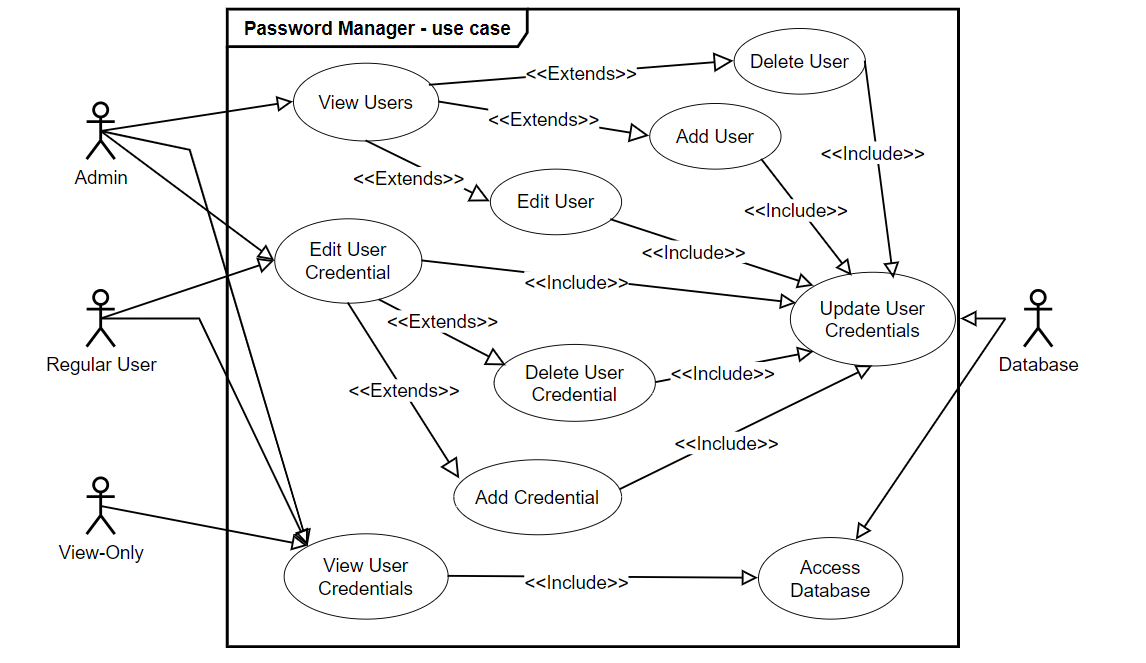
\includegraphics[width=\linewidth]{UseCaseDiagramUpdate.png}
\caption{User perspective use case diagram.}
\label{Usecase}
\end{figure}

\section{Screen Designs}
%Show mock-ups of the interface from the user's perspective. These can be hand drawn or you can use a software tool to create illustrations. Just make them as accurate as possible. Graph paper works well when hand drawing the screens.

An Illustration of the proposed system was constructed using Axure Software. The illustration of the login screen for all classes of users is displayed in Figure~\ref{Login}. The illustration of an individual credential screen for the view-only user class is displayed in Figure~\ref{IndivCred_VU}. The illustration of an individual credential screen for both the admin and regular user classes is displayed in Figure~\ref{IndivCred_RAU}. An illustration of the stored credentials list for a view-only user is displayed in Figure~\ref{CredList_VU}. An illustration of the stored credentials list for a regular user is displayed in Figure~\ref{CredList_RU}. An illustration of the stored credentials list for a admin user is displayed in Figure~\ref{CredList_AU}. The illustration of the user management screen to allow an admin user to create, edit, and delete users is displayed in Figure~\ref{UserManagment}.

\begin{figure}
\centering
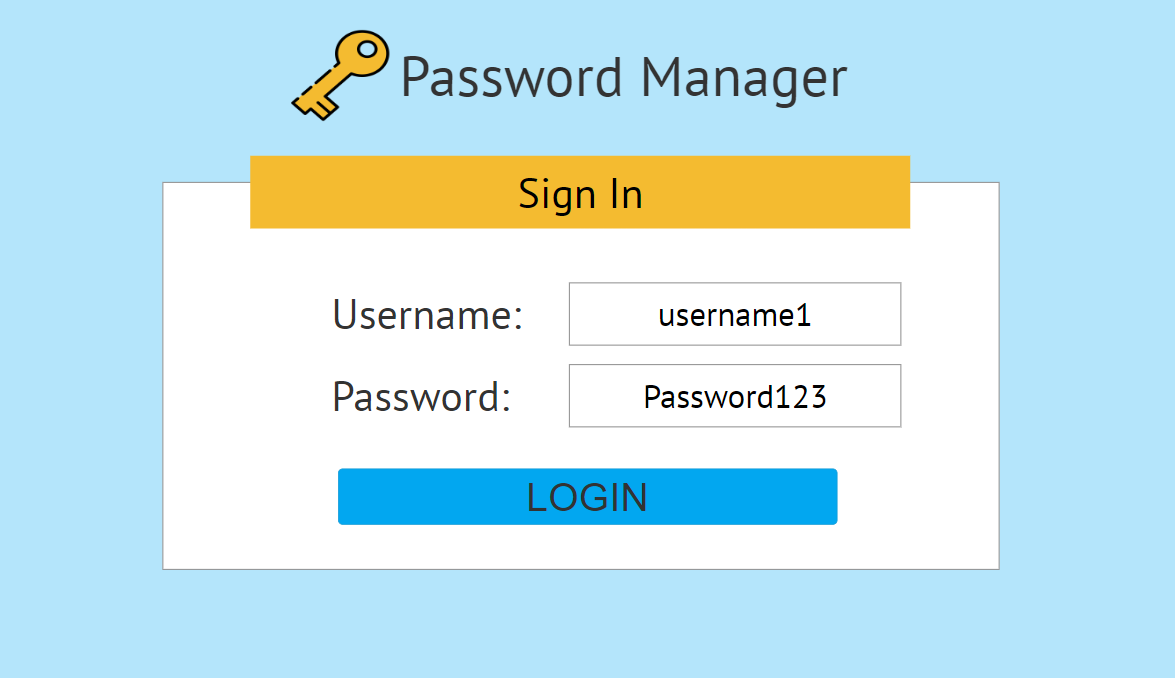
\includegraphics[width=\linewidth]{UI_login.png}
\caption{Login Illustration for All Users}
\label{Login}
\end{figure}

\begin{figure}
\centering
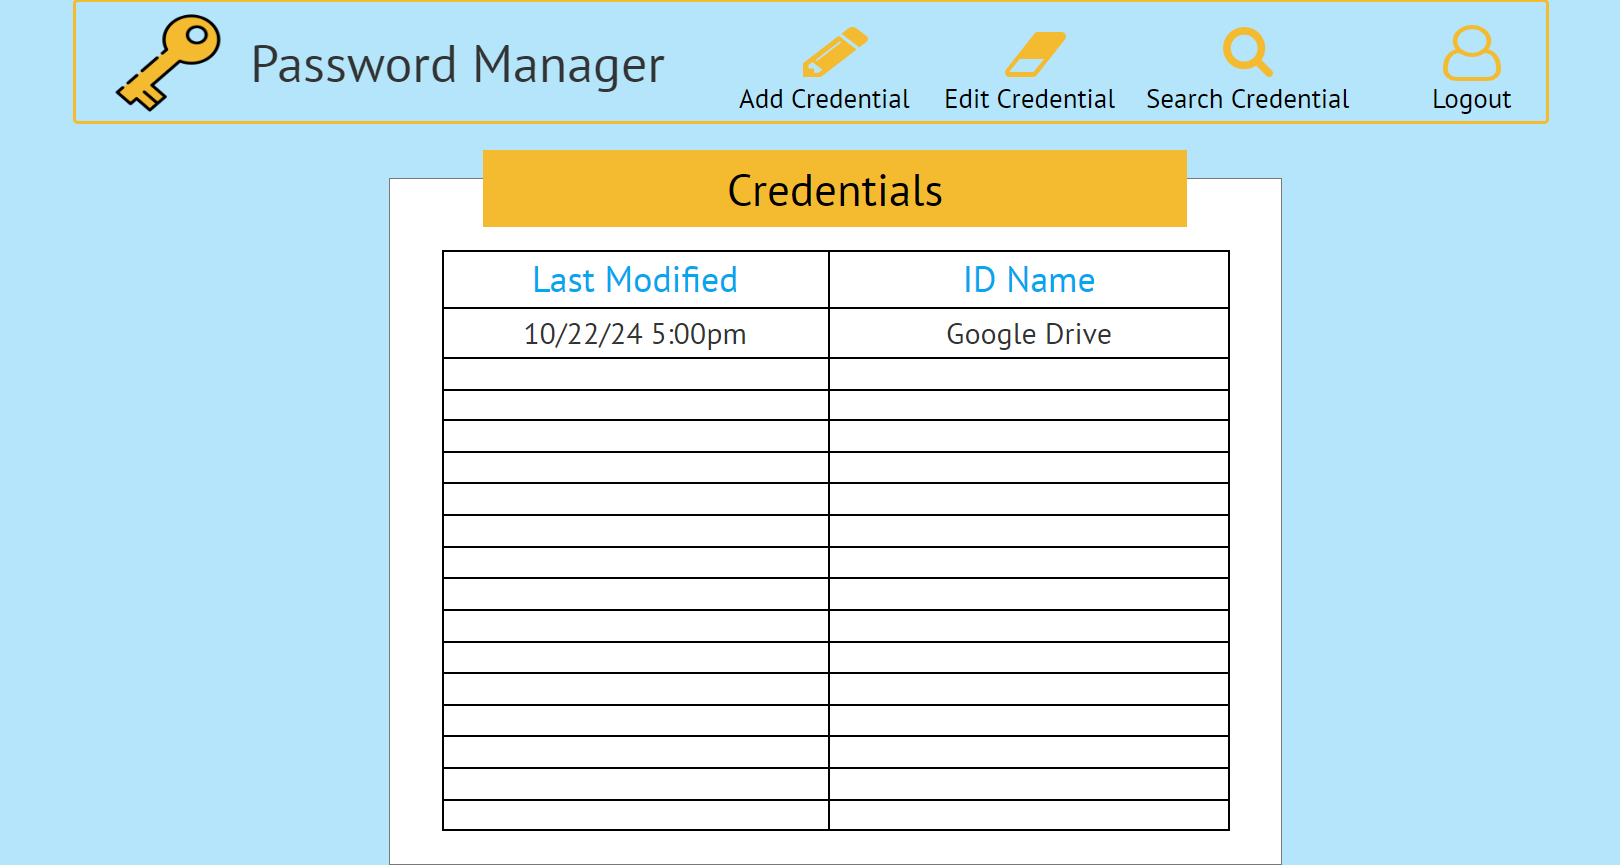
\includegraphics[width=\linewidth]{NewUI.png}
\caption{Credentials List Illustration for Regular User Class}
\label{CredList_RU}
\end{figure}

\begin{figure}
\centering
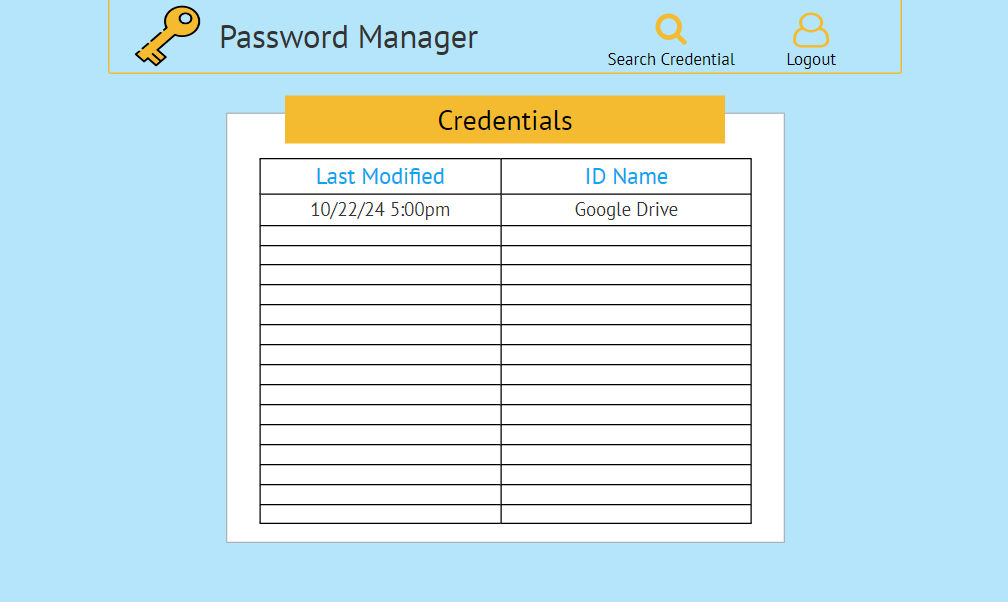
\includegraphics[width=\linewidth]{UI_CredentialList_VO.png}
\caption{Credentials List Illustration for View User Class}
\label{CredList_VU}
\end{figure}

\begin{figure}
\centering
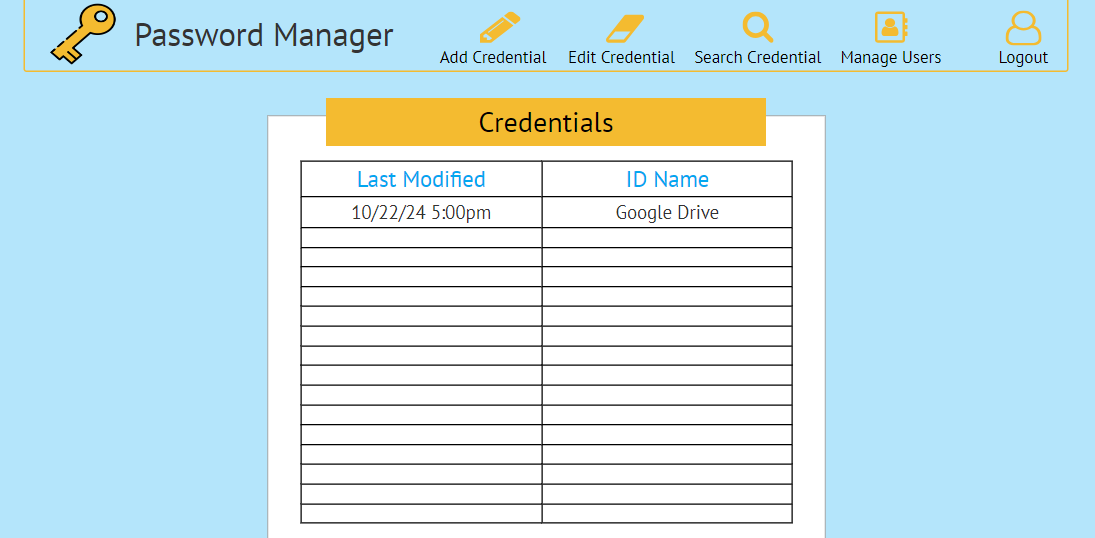
\includegraphics[width=\linewidth]{UI_CredentialList_A.png}
\caption{Credentials List Illustration for Admin User Class}
\label{CredList_AU}
\end{figure}

\begin{figure}
\centering
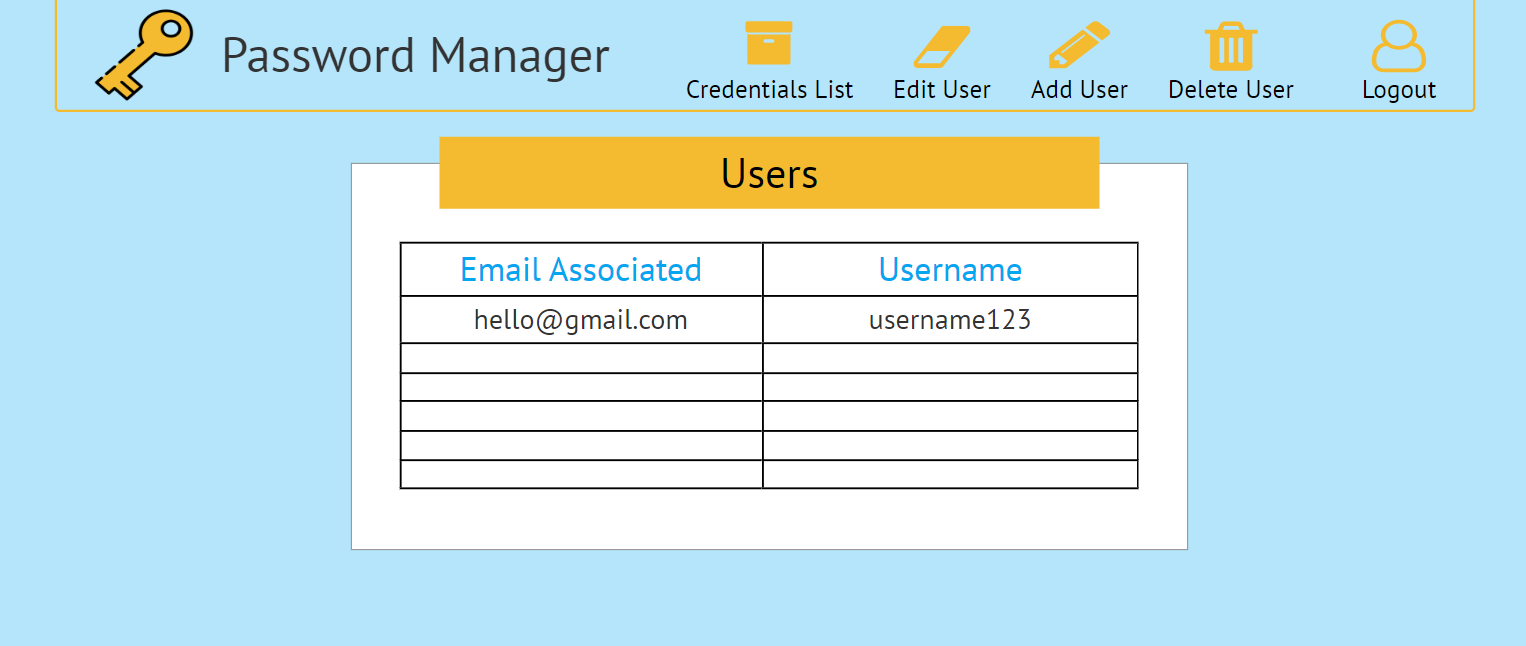
\includegraphics[width=\linewidth]{UI_UserManagement.png}
\caption{User Management Page Illustration for Admin User Class}
\label{UserManagment}
\end{figure}

\begin{figure}
\centering
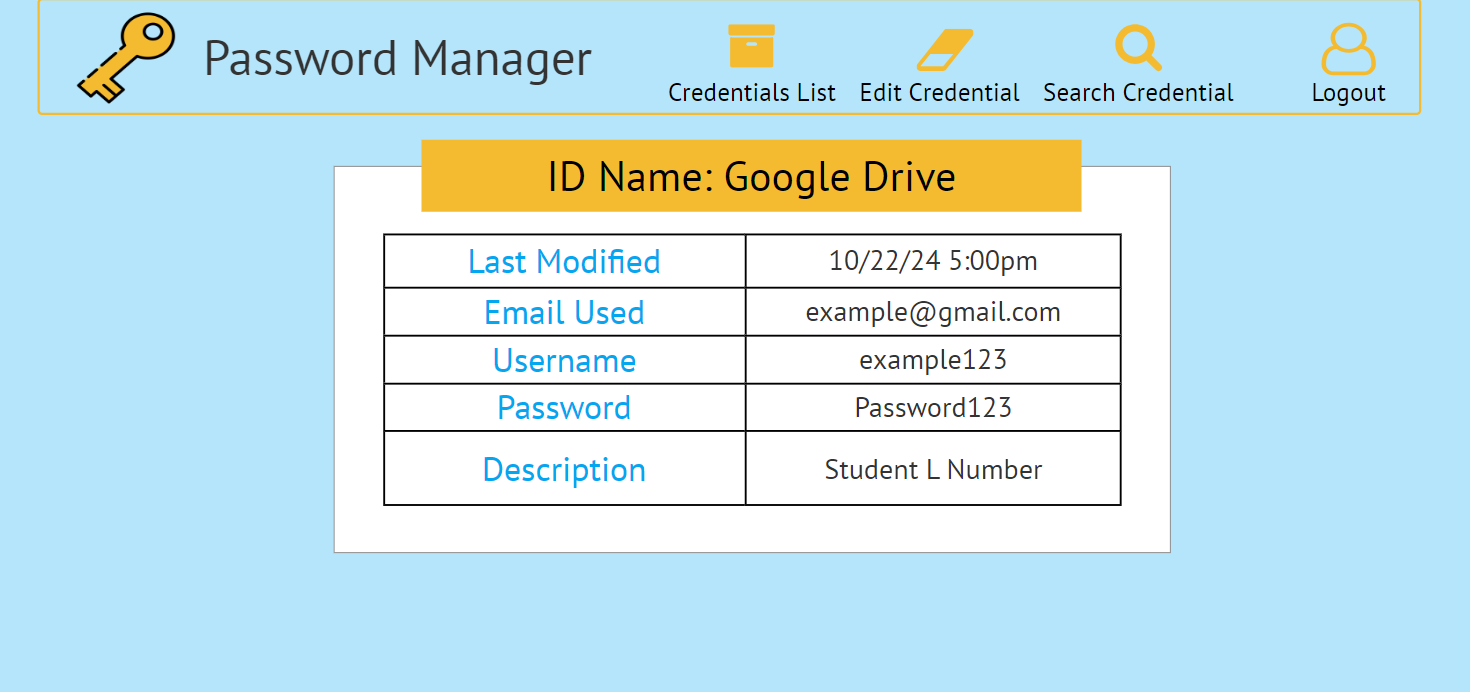
\includegraphics[width=\linewidth]{UI_Credential.png}
\caption{Individual Credential Illustration for Regular and Admin User Classes}
\label{IndivCred_RAU}
\end{figure}

\begin{figure}
\centering
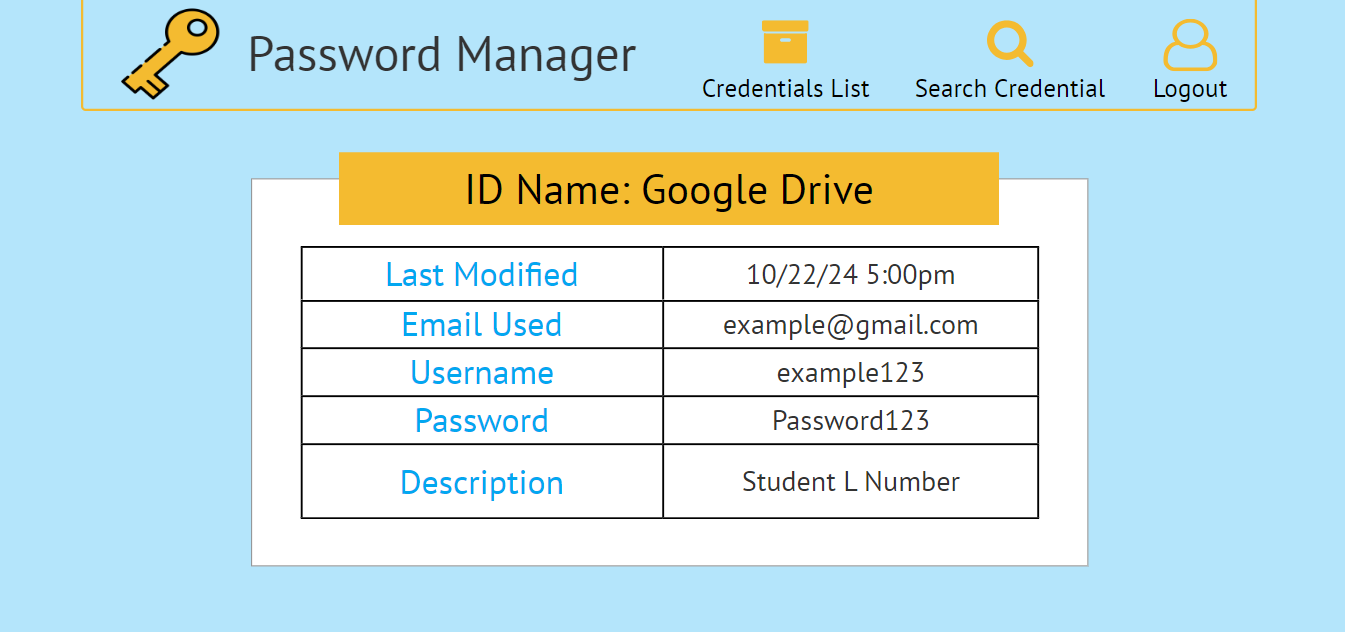
\includegraphics[width=\linewidth]{UI_Credential_VO.png}
\caption{Individual Credential Illustration for View User Class}
\label{IndivCred_VU}
\end{figure}

\chapter{REQUIREMENTS MATRIX} % a.k.a. RTVM (requirements traceability verification matrix)
%Provide a cross-reference that traces each component and data structure to the requirement(s) in the SRS document. Use a tabular format to show which system components satisfy each one of the functional and non-functional requirements. Refer to the requirements by the number/code used in the SRS document.

\begin{table}[h]
\centering
\begin{tabularx}{\textwidth}{|l|X|X|l|}
\hline
\textbf{Requirement-ID} & \textbf{Requirement Description} & \textbf{Design Component} & \textbf{Test-Case \#} \\
\hline
\multicolumn{4}{|l|}{\textbf{Performance Requirements}} \\
\hline
R1.1 & The software shall support 10 users while maintaining a maximum response time of 2 seconds. & System Architecture & T1 \\
\hline
R1.2 & The software shall exhibit response times of between 0-2 seconds after user input. & User Interface & T2 \\
\hline
R1.3 & Unplanned extended downtime shall not exceed 1 minute each week. & Server Infrastructure & T3 \\
\hline
R1.4 & The software shall support a minimum of two users altering credentials at the same time. & Authentication Module & T4 \\
\hline
\end{tabularx}
\caption{Requirements Traceability Verification Matrix - Performance Requirements}
\label{tab:RTVM1}
\end{table}

\begin{table}[h]
\centering
\begin{tabularx}{\textwidth}{|l|X|X|l|}
\hline
\textbf{Requirement-ID} & \textbf{Requirement Description} & \textbf{Design Component} & \textbf{Test-Case \#} \\
\hline
\multicolumn{4}{|l|}{\textbf{Security Requirements}} \\
\hline
R3.1 & Admin passwords shall not be obtainable by any user but that specific admin. & Encryption Module & T5 \\
\hline
R3.2 & Data log access shall only be available to Admin users. & Access Control & T6 \\
\hline
R3.3 & All data transfers containing user data shall be encrypted. & Encryption Module & T7 \\
\hline
R3.4 & Sessions shall expire after an inactivity of 30 minutes. & Session Manager & T8 \\
\hline
R3.5 & The software shall enforce password authentication requirements following the NIST Digital Identity Guidelines (SP 800-63B). & Compliance Module & T9 \\
\hline
R3.6 & Accounts shall lock after three repeated failed login attempts. & Authentication Module & T10 \\
\hline
R3.7 & For any database login, a minimum of AES encryption shall be used before authentication. & Database Security & T11 \\
\hline
R3.8 & The software shall prevent data loss of user credentials by completing daily backups of all files to a secondary location. & Backup System & T12 \\
\hline
R3.9 & All interactions with the database shall access the database with the least privilege possible for the least amount of time. & Database Access Control & T13 \\
\hline
\end{tabularx}
\caption{Requirements Traceability Verification Matrix - Security Requirements}
\label{tab:RTVM2}
\end{table}

\begin{table}[h]
\centering
\begin{tabularx}{\textwidth}{|l|X|X|l|}
\hline
\textbf{Requirement-ID} & \textbf{Requirement Description} & \textbf{Design Component} & \textbf{Test-Case \#} \\
\hline
\multicolumn{4}{|l|}{\textbf{Software Quality Attributes}} \\
\hline
R4.1 & The software shall be divided into a minimum of 2 components that can be modified individually. & Modular Design & T14 \\
\hline
R4.2 & Components shall allow the ability to update without affecting other parts of the system. & Modular Design & T15 \\
\hline
R4.3 & Software shall be accompanied by documentation. & Documentation & T16 \\
\hline
R4.4 & The software shall protect against unauthorized access and data breaches. & Security Framework & T17 \\
\hline
\end{tabularx}
\caption{Requirements Traceability Verification Matrix - Software Quality Attributes}
\label{tab:RTVM3}
\end{table}


\end{document}
sdd.tex
9 KB
